% ==== [sudoer] MORE PORCELAIN ====
\section{\emph{[sudoer]} More porcelain}

\begin{frame}[fragile]{Save/Restore a dirty working directory}
  \texttt{git-stash(1)} saves the current state of the working directory + the index, and goes back to a clean WD.

  Saved changes can be restored with {\ttfamily\scriptsize\$ git stash pop}. Git-stash stack can be dumped by {\ttfamily\scriptsize\$ git stash list}.
  \pause

  \begin{lstlisting}[style=bash]
    $ echo foo > README.md
    $ git status
    On branch foo
    Changes not staged for commit:
    ``        `{\color{cred}modified:   README.md}\pause`

    $ git stash
    Saved working directory and index state WIP on foo: 9f7f586 README.md has been added
    $ git status
    On branch foo
    nothing to commit, working tree clean`\pause`

    $ git stash pop
    On branch foo
    Changes not staged for commit:
    ``        `{\color{cred}modified:   README.md}`
    Dropped refs/stash@{0} (35365e0c188e877ded1ecdd8190ec5bb1b6c2c1b)
  \end{lstlisting}
\end{frame}

\begin{frame}{Applying changes from other branches}
  \begin{columns}
    \column{.55\textwidth}
    \texttt{git-cherry-pick(1)} apply the changes introduced by the given commits, e.g.\par
    {\ttfamily\scriptsize\$ git cherry-pick 9f7f586}.\\[1em]
    The patch may not apply cleanly; if that is the case, you are required to resolve conflicts

    \column{.45\textwidth}
    \centering
    \tikz[every label/.style={font=\tiny}]{
      \graph[tree layout,grow'=up,nodes={simple commit obj,as=}]
            { a <- aa <- { b <- bb <- bbb[mLightBrown,label=left:9f7f586] <- bbbb[label=90:master],
                          c <- cc }
            };
      \draw<2>[<-] (cc) -- ++(0em,2.6em)
                   node(ccc)[simple commit obj,mLightBrown83,label=right:0c151e4]{};
      \foreach \i [count=\c] in {cc,ccc} \path<\c> node[above=0pt of \i,font=\tiny]{foo};
    }
  \end{columns}
\end{frame}

{
\tikzset{every label/.style={font=\tiny},
        commit 1/.style={simple commit obj,fill=teal},
        commit 2/.style={simple commit obj,fill=teal!74},
        commit 3/.style={simple commit obj,fill=teal!56}}
\begin{frame}{Rebasing (1/3)}
  A long-lived branch may become outdated w.r.t. its parent. Naïve approach: merge in the parent branch.\par
  \begin{center}
    \tikz[hole/.style={densely dotted},
          merge/.style={simple commit obj,mLightBrown}]{
      \graph[tree layout,grow'=right,nodes={simple commit obj,as=}] {
        a <- aa[red] <- { [nudge down=3ex] b[label=above:A] <- bb[label=above:B] <- bbb[label=above:C] }
      };
      \draw<2->[<-] (aa) -- ++(3ex,3ex) node(c)[commit 1]{} -- ++(3ex,0ex) node(cc)[commit 2]{};
      \draw<2->[hole] (cc) -- ++(5ex,0ex) node(ccc)[commit 3]{};
      \draw<3->[<-] (bbb) -- ++(5ex,0ex) node(bbbb)[merge]{}
                    (ccc) -- (bbbb);
      \draw<4->[hole] (ccc) -- ++(10ex,0ex) node(cccc)[simple commit obj]{}
                    (bbbb) -- ++(10ex,0ex) node(bbbbb)[merge]{};
      \draw<4->[<-] (cccc) -- (bbbbb);
      % branch heads
      \foreach \i/\j/\k in {1/aa/master,1-2/bbb/topic,
                          2-3/ccc/master, 3/bbbb/topic,
                          4/cccc/master,4/bbbbb/topic}
        \path<\i> node[right=0pt of \j,font=\tiny]{\k};
    }
  \end{center}
  
  \onslide<5>{
    This clutters project history. Reapplying \texttt{topic} commits on top of \texttt{master} is better!\par
    \begin{center}
    \tikz\graph[tree layout,grow'=right,nodes={simple commit obj,as=}] {
        a <- aa[red] <- c[commit 1] <- cc[commit 2] <- ccc[commit 3,label=right:master]
            <- { [nudge down=3ex] b[label=above:A'] <- bb[label=above:B'] <- bbb[label=above:C',label=right:topic] }
      };
    \end{center}

    \tikz\node[TTfamily]
              {{\color{cyellow}\# Assuming that 'topic' is the current branch, this gives the result above}\\
              \$ git rebase master};
  }
\end{frame}

\begin{frame}{Rebasing (2/3)}
  It is one of the most powerful Git commands, as it can be used to rewrite project history.\par
  If there are conflicts, you will have to resolve them (as in merge).\pause

  \warning{\texttt{GIT-REBASE(1)} IMPLICATIONS:}
  \begin{itemize}
  \item Requires rewriting commits and is \alert{PROBLEMATIC} if you already pushed those objects
  \item You can break things: \alert{YOU HAVE BEEN WARNED!}
  \item If you ever force-push a rebased branch, others will have to fix their history. See git-rebase(1), section ``RECOVERING FROM UPSTREAM REBASE''.
  \end{itemize}
\end{frame}

\begin{frame}[fragile]{Rebasing (3/3)}
  \texttt{git-rebase(1)} has an interactive mode in which you can edit/reorder/remove the commits, e.g.

  \begin{onlyenv}<1>
    \begin{center}
      \tikz\graph[tree layout,grow'=right,nodes={simple commit obj,as=}] {
        a <- aa[red] <- { c <- cc[label=right:master],
            b <- bb[label=below:\LT after-this-commit\GT]
              <- bbb[commit 1,label=above:A] <- bbbb[commit 2,label=above:B] <- bbbbb[commit 3,label=above:C,label=right:topic] }
      };
    \end{center}
    \begin{lstlisting}[style=bash]
      # This fires up an editor and gives you the chance to edit the commit list
      $ git rebase -i <after-this-commit>
    \end{lstlisting}

    \gitRebaseWarning
  \end{onlyenv}

  \only<2->{
    \centering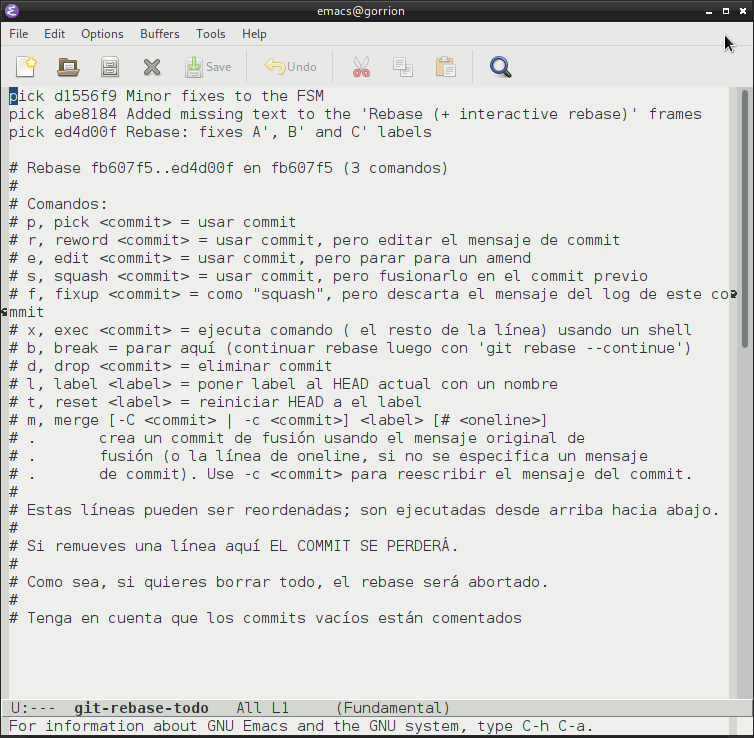
\includegraphics[height=.78\textheight]{img/git-rebase_-i.png}
  }

  \only<3->{
    \hintBox{In an scenario with stacked branches, you probably want to rebase the top-most branch and use the \texttt{--update-refs} option.}
  }
\end{frame}
}

\begin{frame}[fragile]{More about fixing history (1/2)}
  So common that \texttt{git-commit(1)} has \texttt{--squash} and \texttt{--fixup} to mark commits to be automatically squashed.\par
  Rewriting occurs during {\ttfamily\scriptsize\$ git rebase --autosquash}.
  \pause
  \begin{lstlisting}[style=bash]
    $ git log --oneline
    e7a2019 (HEAD -> master) Any other changes
    9f7f586 Added README.md
    02a7fb9 Added bar.txt`\pause`

    $ echo foo >> README.md && git commit -a --fixup 9f7f586
    $ git log --oneline
    24a54df (HEAD -> master) fixup! Added README.md
    e7a2019 Any other changes
    9f7f586 Added README.md
    02a7fb9 Added bar.txt`\pause`

    $ git rebase -i --autosquash 02a7fb9
    Successfully rebased and updated refs/heads/master.
    $ git log --oneline
    528efb7 (HEAD -> master) Any other changes
    a59735c Added README.md
    02a7fb9 Added bar.txt
  \end{lstlisting}
\end{frame}

\begin{frame}{More about fixing history (2/2)}
  If you only need to rewrite the last commit use\\ {\ttfamily\scriptsize\$ git commit --amend}

  \gitRebaseWarning
\end{frame}

\begin{frame}{git filter-branch}
  \Q I know how to rewrite commits. Can I automate the process?\\
  \pause
  \A \texttt{git-filter-branch(1)}\footnote{See also \texttt{git filter-repo}.} lets you rewrite branches, applying filters to modify each tree/information about each commit, e.g. \\[1em]

  \tikz\node[TTfamily]
            {\$ git log --oneline\\
            {\color{cyellow}92cb761} (HEAD -\GT{} foo) Added nsswitch.conf\\
            {\color{cyellow}9f7f586} Added README.md\\
            {\color{cyellow}02a7fb9} (bar) Added bar.txt\\[1ex]
            \$ git filter-branch --msg-filter 'sed -e "s/Added \textbackslash([[:graph:]]*\textbackslash)\$/\textbackslash{}1 has been added/"' foo\\[1ex]
            \$ git log --oneline\\
            {\color{cyellow}6e9fbd6} (HEAD -\GT{} foo) nsswitch.conf has been added\\
            {\color{cyellow}63feb3c} README.md has been added\\
            {\color{cyellow}2fe54f3} bar.txt has been addded};

  \gitRebaseWarning
\end{frame}

\begin{frame}[fragile]{I messed things up!  Help!}
  If you broke something (e.g. after a \texttt{git rebase} or \texttt{git filter-branch}), you can see how a particular ref was updated and revert to a previous state, e.g.

  \begin{lstlisting}[style=bash]
    $ git reflog my-branch
    cb96893 (HEAD -> master) master@{0}: rebase (finish): refs/heads/master onto 5cfbdfa884cb0b0830006f363b406a99458c0f10
    `{\color{cyellow}ec09a4e}` master@{1}: commit: Add license file    `{\color{red}$\leftarrow$ Before the rebase}`
    f922003 master@{2}: rebase (finish): refs/heads/master onto 5cfbdfa884cb0b0830006f363b406a99458c0f10
    2193c4b master@{3}: commit: fixup! Update README.md
    `\ldots`

    $ git reset --hard `{\color{cyellow}ec09a4e}`
  \end{lstlisting}
\end{frame}

\begin{frame}{Comparing branches}
  \Q Can I see where each of the given branches is w.r.t. others?\\
  \pause
  \A \texttt{git-show-branch} is your friend. Also, \texttt{git log --graph --oneline \ldots}\\[1em]

  \tikz\node[TTfamily]
            {\$ git show-branch master foo\\
            {\color{cred}!} [master] Added README.md\newline
            \phantom{!}{\color{cgreen}*} [foo] Added nsswitch.conf\newline
            \phantom{!*}{\color{cyellow}!} [bar] Added bar.txt\\
            ---\newline
            \phantom{+}{\color{cgreen}*}\phantom{+} [foo] Added nsswitch.conf\\
            {\color{cred}+}{\color{cgreen}*}\phantom{+} [master] Added README.md\\
            {\color{cred}+}{\color{cgreen}*}{\color{cyellow}+} [bar] Added bar.txt\\[1ex]
            \# To include all remote-tracking and local branches:\\
            \$ git show-branch --all};
\end{frame}

\begin{frame}{Share by other means}
  TAR or ZIP archives of a particular tree can be created by \texttt{git-archive(1)}, e.g.\\[1ex]
    \tikz\node[TTfamily]
            {\$ git archive --format=tar --prefix=foo/ -o foo.tar.gz master};\\[2em]
            
  Git also can generate an archive of packed objects and references to be imported into a repository (useful if machines are not directly connected), e.g.\\[1ex]
    \tikz\node[TTfamily]
            {[alice@earth \~{}]\$ git bundle create /tmp/foo-master.git master\\
            \# /tmp/foo-master.git is copied to moon by some means.\\[1ex]
            [bob@moon \~{}]\$ git clone -b master \~{}/foo-master.git\\[1ex]
            \# Or if the repository already exists\ldots{}\newline
            [bob@moon \~{}]\$ git remote add foo-bundle \~{}/foo-master.git\newline
            [bob@moon \~{}]\$ git pull foo-bundle master};
\end{frame}

\begin{frame}[fragile]{Rerere}
  \texttt{git-rerere} --- Reuse recorded resolution of conflicted merges, i.e. git remembers how you resolved a hunk conflict and it automatically resolves it next time.\\[1em]

  \begin{lstlisting}[style=bash]
    $ git config --global rerere.enabled true
  \end{lstlisting}

  \vfill
  See more at \texttt{git-rerere(1)} manual page, and \href{https://git-scm.com/book/en/v2/Git-Tools-Rerere}{\underline{Git Book, Sec. 7.9 Git Tools - Rerere}}.
\end{frame}
